\documentclass[10pt]{article}
\usepackage[a4paper,margin=1.65cm]{geometry}
\usepackage[T1]{fontenc}
\usepackage{lmodern}
\usepackage{microtype}
\usepackage{amsmath,amssymb}
\usepackage{booktabs}
\usepackage{graphicx}
\usepackage{float}
\usepackage{caption}
\usepackage{subcaption}
\usepackage{xcolor}
\usepackage{hyperref}
\usepackage{enumitem}
\usepackage{multirow}
\usepackage{xspace}
\usepackage{array}

\hypersetup{colorlinks=true, linkcolor=blue!50!black, citecolor=blue!50!black, urlcolor=blue!50!black}
\setlength{\parskip}{3.5pt}
\setlength{\parindent}{0pt}
\captionsetup{font=small,skip=3pt}
\setlist{nosep,leftmargin=*}

\newcommand{\amas}{AMAS3\xspace}
\newcommand{\sas}{SAS\xspace}
\newcommand{\mas}{MAS\xspace}
\newcommand{\tfgrpo}{TF-GRPO\xspace}
\newcommand{\fscore}{token-F1\xspace}
\newcommand{\contain}{contain\xspace}

\title{\textbf{AMAS3: Training-Free Global Policy Optimization for Efficient Multi-Hop QA}}
\author{System Report}
\date{9 May 2026}

\begin{document}
\maketitle

\begin{abstract}
This report documents the AMAS3 branch after the 9 May 2026 optimization pass. The work produced a training-free adaptive RAG system that jointly optimizes a single-agent shortcut and a multi-agent search path. The system first collected an experience library from IRCoT training questions, then ran a TF-GRPO-inspired mixed-dataset policy search over 179 train questions and 8 fixed candidate policies. The optimized policy family rewards answer quality and token efficiency without weight updates, ensembling, majority voting, test labels, or baseline predictions as inference features. On full evaluation, AMAS3 obtains the best exact match and token-F1 among the evaluated no-thinking top-5 baselines on MuSiQue, HotpotQA, 2Wiki, and Bamboogle. TF-GRPO improves HotpotQA from 0.5108 to 0.5286 F1 while reducing mean tokens from 8015 to 7351, and improves 2Wiki from 0.4504 to 0.4638 F1 at nearly unchanged token cost. MuSiQue and Bamboogle keep their compact base policies because the train-time search did not find a better validated full-run Pareto point.
\end{abstract}

\section{Problem setting}

The research objective was to move beyond a static multi-agent RAG pipeline. The desired system should be adaptive: easy questions should exit through a cheap single-agent path, while harder compositional questions should invoke decomposition, focused retrieval, solver calls, repair, and synthesis. The practical constraint was equally important: the method had to stay around the 6k to 9k token range on full datasets, and optimization had to be training-free.

The design constraints were strict. The system could not ensemble independent generations, pool answers, use majority voting, run best-of-N selection, or use benchmark-specific answer hacks. It also could not use gold answers, OPERA predictions, or baseline outputs as runtime features. Gold answers are used only for offline training-set reward computation and offline evaluation, as in standard validation.

The resulting method is best understood as policy optimization over the inference program. The model weights stay fixed. TF-GRPO trains neither the generator nor the retriever. Instead, it evaluates a group of hand-specified, research-motivated policies on training questions, scores them with a quality and efficiency reward, extracts lessons into an experience library, and chooses a deterministic deployment profile.

\section{AMAS3 architecture}

\paragraph{Two-lane execution.}
AMAS3 has a cheap single-agent lane and a multi-agent lane. The single-agent lane retrieves a small evidence set and tries to answer directly. If this path is sufficiently grounded and type-aligned, the system can exit early. Otherwise, the multi-agent lane is used.

The multi-agent lane contains four functional stages:
\begin{enumerate}
  \item \textbf{Planner}: decomposes the question into a limited number of subgoals.
  \item \textbf{Focused retriever and solver}: retrieves evidence for each subgoal and extracts a short answer span.
  \item \textbf{Repair and alignment}: checks whether the answer addresses the original question, especially for comparison cases.
  \item \textbf{Synthesizer}: combines the strongest evidence and emits the final answer.
\end{enumerate}

\paragraph{Main implementation changes.}
The branch added budget-aware control to the planner, solver, and synthesizer. The planner now supports a maximum subgoal cap. The solver receives the original question during answer-span extraction and query rewrite, which prevents subgoal-local answers from overwriting the final target. The synthesizer now supports compact evidence windows, no-chain-of-thought operation, and a skip condition when the solver has already produced a high-confidence answer.

\paragraph{Comparison alignment.}
A concrete failure mode appeared in HotpotQA and 2Wiki: the solver often found the compared value but returned the value instead of the candidate associated with it. For example, a comparison question may ask which entity has the larger population, while an intermediate solver returns the numeric population. AMAS3 now includes deterministic comparison alignment. It extracts candidates from the question and evidence trail, maps observed values back to candidates, and only changes the final answer when the mapping is direct. This is not answer voting and does not introduce new candidate answers.

\section{Experience library collection}

The first stage was deliberately small and diagnostic. AMAS3 ran four initial policies on 36 IRCoT training questions, producing 144 rollouts. The set mixed MuSiQue, HotpotQA, and 2Wiki examples. Each rollout stored the question source, policy name, predicted answer, gold answer for offline scoring, F1, contain, reward, actual token usage, number of subgoals, retrieval calls, solver calls, topology, and wall-clock time.

The initial library was not a prompt-only memory. It was a structured trace summary of what happened when different policies spent tokens in different ways. The library recorded policy statistics, source-specific policy statistics, over-budget counts, zero-F1 counts, and compact natural-language lessons. Table~\ref{tab:library} summarizes the first pass.

\begin{table}[H]
\centering
\small
\begin{tabular}{lrrrrr}
\toprule
Initial policy & Train rollouts & Mean F1 & Mean contain & Mean tokens & Zero-F1 \\
\midrule
compact5 synthesis & 36 & .408 & .333 & 6573 & 19 \\
compact fast-final & 36 & .371 & .306 & 5583 & 21 \\
compact synthesis & 36 & .433 & .361 & 6976 & 18 \\
full reference & 36 & .405 & .333 & 9982 & 19 \\
\bottomrule
\end{tabular}
\caption{Initial experience-library collection over 36 IRCoT training questions and four policies. The full reference policy spent many more tokens without a reliable quality gain, which motivated compact synthesis and stronger answer alignment.}
\label{tab:library}
\end{table}

The initial library produced five operational lessons that shaped the later search. First, SAS should be used only as a verifier-gated cheap exit. Second, most questions should use compact MAS plans with at most three subgoals. Third, broad 20-chunk synthesis burns tokens without consistent F1 gains. Fourth, fast-final saves tokens but can lose target alignment. Fifth, comparison questions require preserving the requested candidate or class as the final answer, not returning the compared property.

This library is the ``experience'' component in the method. It is not used as a set of candidate answers. It is a control memory that tells the policy search which system dimensions are worth varying and which failure modes should be repaired.

\section{What TF-GRPO optimizes}

\paragraph{Training-free meaning.}
TF-GRPO is used here as a group-relative policy-selection procedure over inference configurations. It does not update model weights. It trains the controller in the sense that it chooses a better inference policy from rollouts, then freezes that policy for evaluation.

\paragraph{Training data.}
The main global search used 179 IRCoT training questions: 69 MuSiQue, 57 HotpotQA, and 53 2Wiki. These are train questions only. The full evaluation sets were not used for policy reward computation. The search evaluated 8 policies on every training question, giving 1432 rollouts.

\paragraph{Reward.}
Each rollout produces a prediction and actual token count. The reward combines answer quality and efficiency:
\begin{equation}
q = 0.75 \cdot \text{F1} + 0.25 \cdot \text{contain},
\end{equation}
\begin{equation}
R = q - \lambda \cdot \min(t / T, 2.0),
\end{equation}
where $t$ is actual total tokens, $T$ is the token target, and $\lambda$ is the token penalty weight. The final global run used a target near 8500 tokens and a moderate efficiency penalty. This reward prefers concise policies only when they preserve answer quality. It also prevents the search from choosing the old high-context policy simply because it gives the model more room to reason.

\paragraph{Group-relative selection.}
For each training question, all candidate policies are evaluated. The procedure then computes both aggregate mean reward and per-question winner counts. Mean reward identifies robust average policies. Winner counts identify policies that frequently dominate within question groups. The final selection is not a majority vote at inference time. It is an offline comparison of fixed policies on train questions.

\section{Candidate policies}

The candidate policies vary only the system control surface. The axes are retrieval budget, planner depth, synthesis evidence budget, synthesis reasoning mode, and repair. Table~\ref{tab:policies} gives the policy grid.

\begin{table}[H]
\centering
\small
\begin{tabular}{lrrrrccp{4.8cm}}
\toprule
Policy & Ret. & Subgoals & Chunks & Chars & CoT & Repair & Intended behavior \\
\midrule
compact synthesis & 2 & 3 & 8 & 420 & no & no & Default compact MAS with moderate synthesis context. \\
compact5 synthesis & 2 & 3 & 5 & 300 & no & no & Aggressively short synthesis for efficiency. \\
retrieval3 compact8 & 3 & 3 & 8 & 420 & no & no & Extra retrieval attempts without larger synthesis. \\
quality8 repair & 3 & 4 & 8 & 420 & no & yes & Quality-biased policy with one repair pass. \\
CoT retrieval3 compact8 & 3 & 3 & 8 & 420 & yes & no & Tests whether synthesis reasoning helps. \\
quality12 retrieval3 & 3 & 4 & 12 & 500 & no & no & Larger evidence budget without repair. \\
plan6 retrieval3 compact8 & 3 & 6 & 8 & 420 & no & no & Deeper planning for bridge-heavy questions. \\
plan6 retrieval3 oldlike & 3 & 6 & 20 & 700 & yes & yes & High-context reference style. \\
\bottomrule
\end{tabular}
\caption{Policy search space. TF-GRPO optimizes these inference-program choices, not neural weights.}
\label{tab:policies}
\end{table}

\begin{figure}[H]
\centering
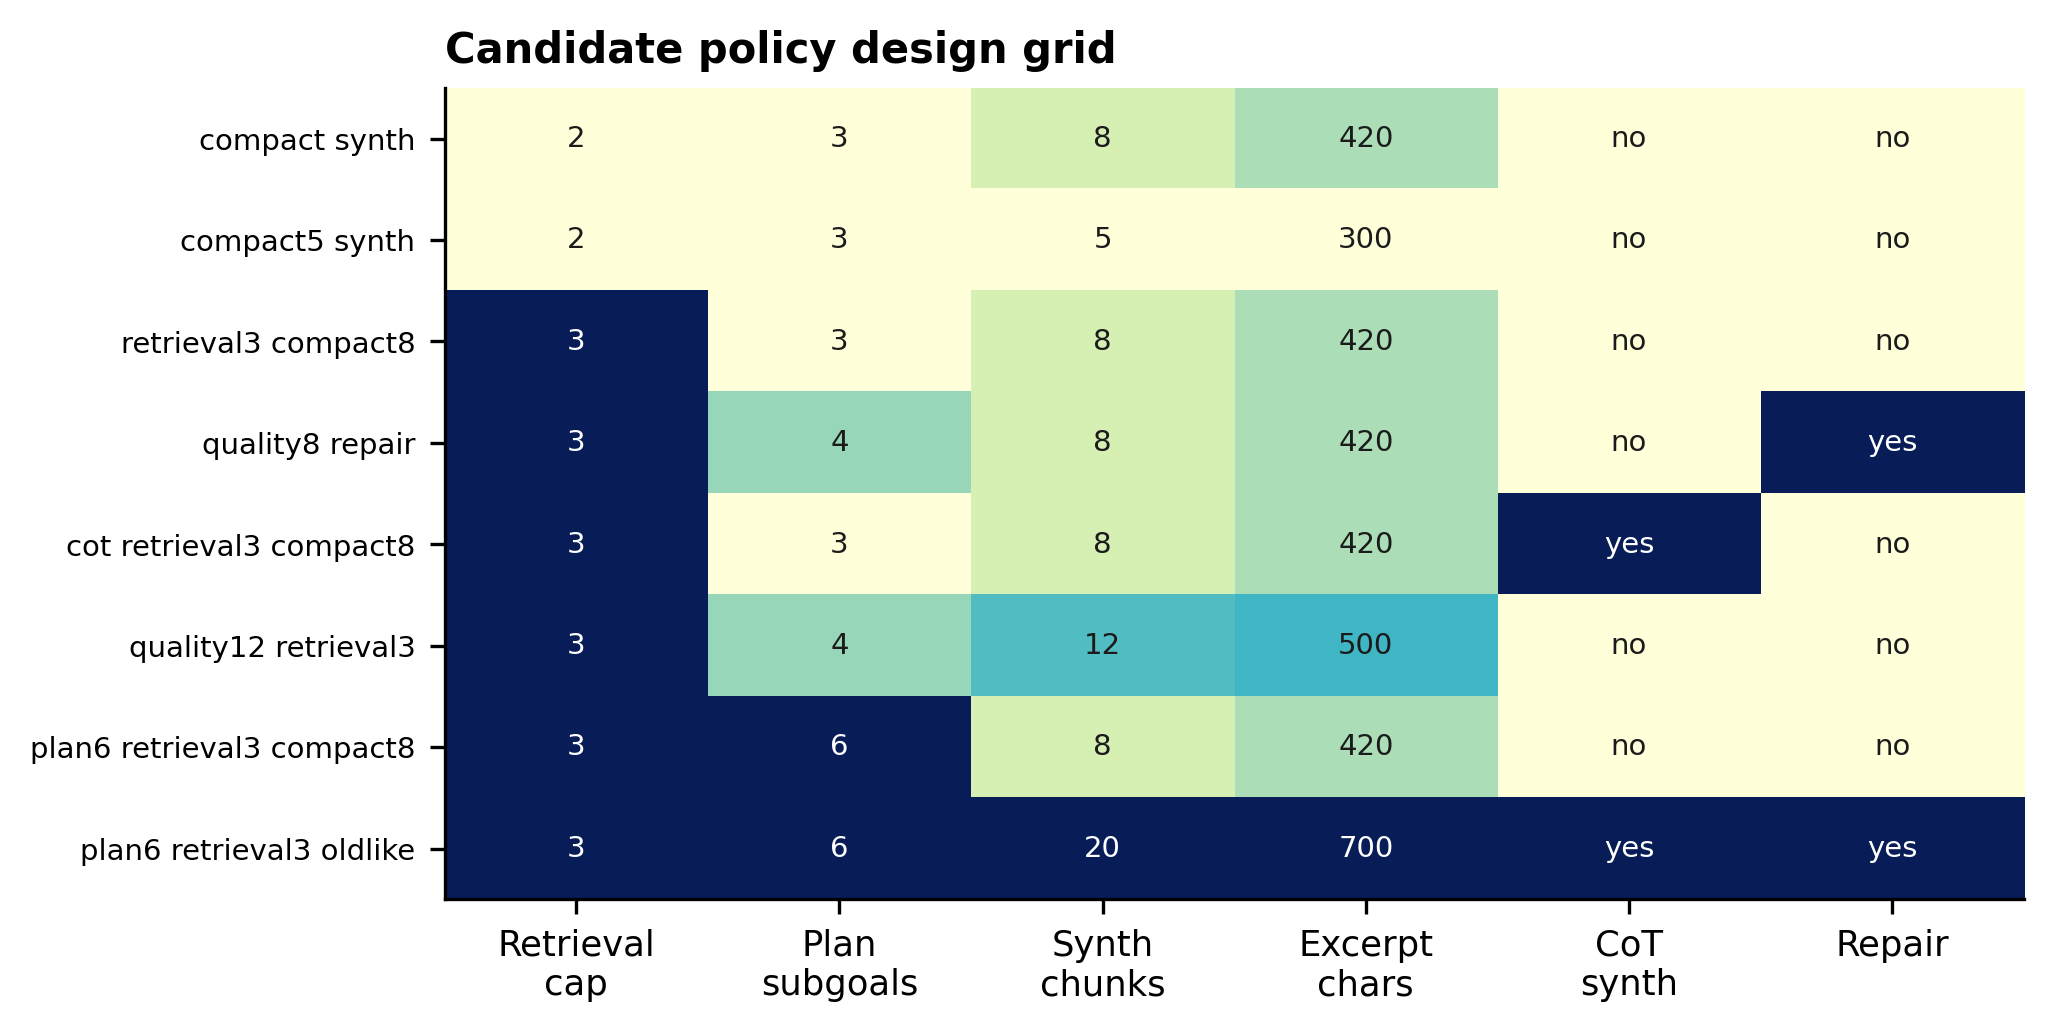
\includegraphics[width=.82\linewidth]{figs/policy_design_grid.png}
\caption{Candidate policy design grid. Darker cells indicate larger normalized control values. The search deliberately spans compact, retrieval-heavy, repair-heavy, deeper-plan, and old high-context regimes.}
\label{fig:policy-grid}
\end{figure}

\section{Mixed-train optimization results}

Figure~\ref{fig:policy-heatmap} shows the source-specific policy surface from the 179-question mixed train search. The annotations show F1 and token usage, while color shows the scalar reward. The important result is that no single axis dominates across all datasets.

\begin{figure}[H]
\centering
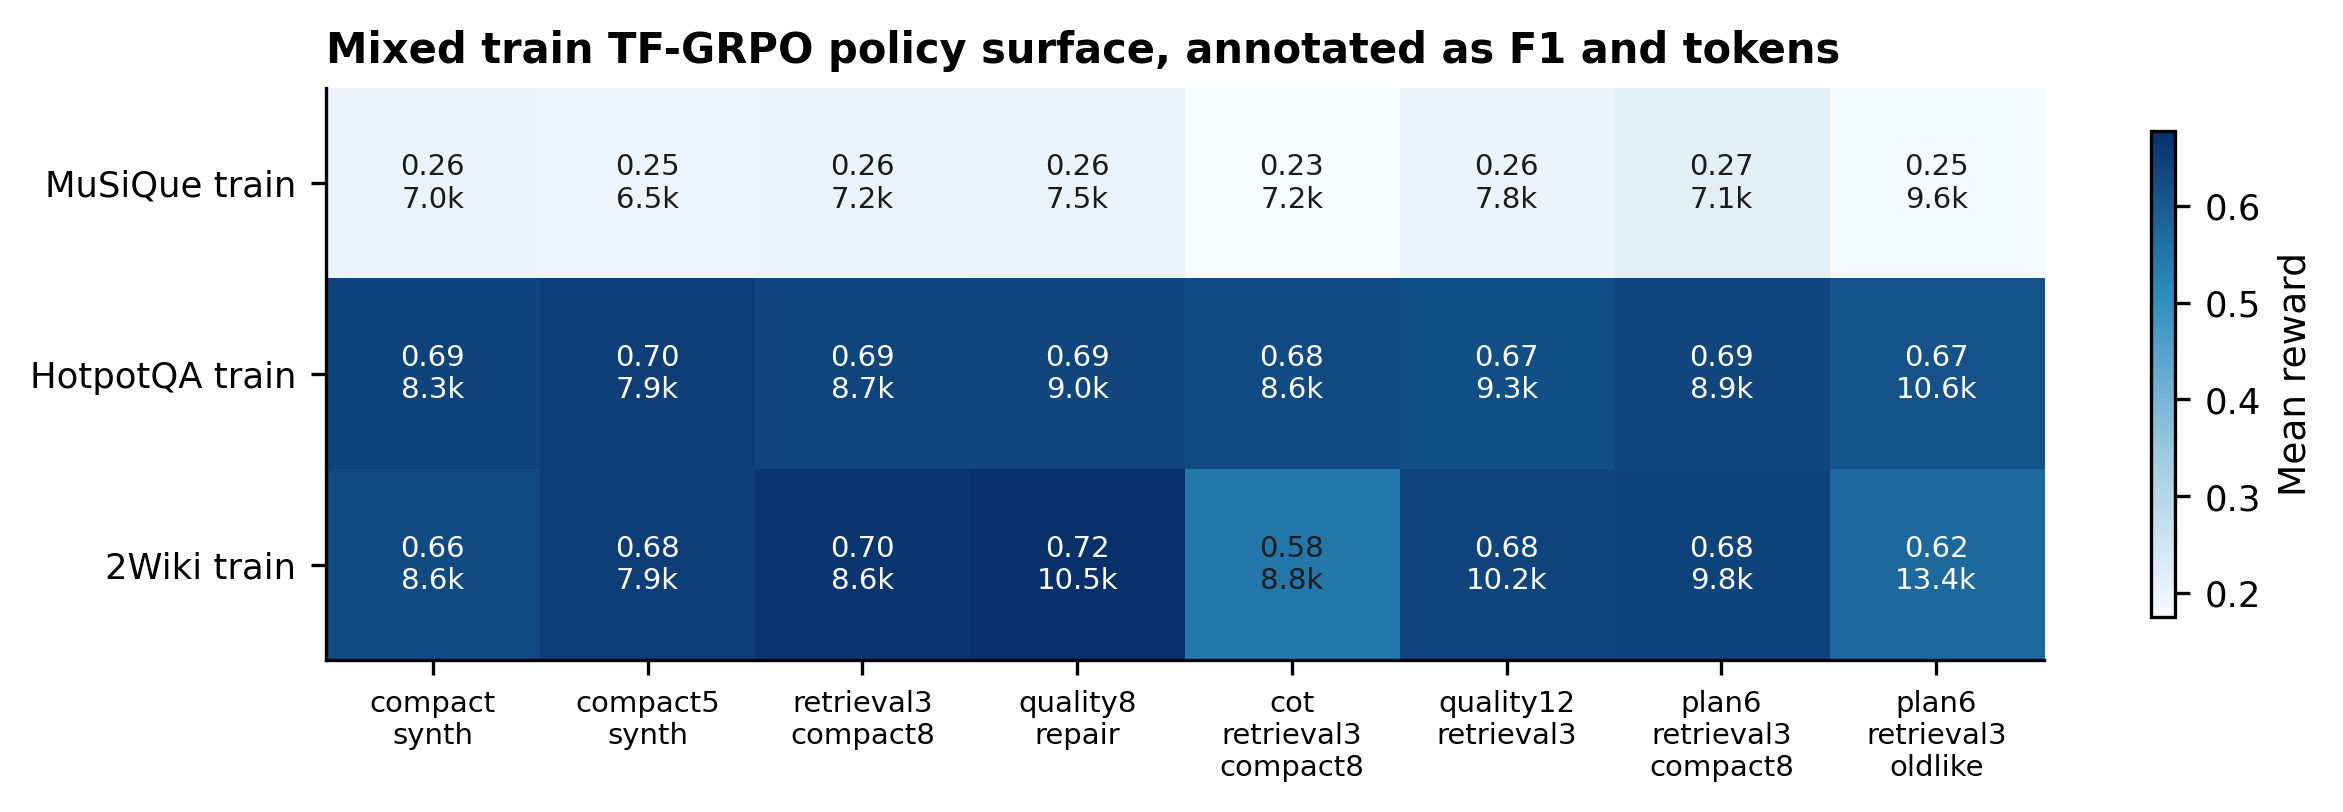
\includegraphics[width=.96\linewidth]{figs/policy_reward_heatmap.png}
\caption{Mixed-train TF-GRPO policy surface. HotpotQA preferred compact synthesis, 2Wiki benefited from quality and repair, and MuSiQue preferred deeper planning with extra retrieval.}
\label{fig:policy-heatmap}
\end{figure}

The global mean-reward winner was the quality repair policy, but the compact five-evidence synthesizer won the most individual train questions. The interpretation is useful: compact synthesis is the safest general policy, while repair is valuable when the dataset has many comparison and candidate-alignment failures.

\begin{table}[H]
\centering
\small
\begin{tabular}{lrrrrr}
\toprule
Policy & Mean reward & Train F1 & Train contain & Tokens & Wins \\
\midrule
compact synthesis & .468 & .515 & .475 & 7917 & 5 \\
compact5 synthesis & .475 & .520 & .480 & 7384 & 162 \\
retrieval3 compact8 & .478 & .526 & .486 & 8090 & 3 \\
quality8 repair & .480 & .532 & .492 & 8885 & 3 \\
CoT retrieval3 compact8 & .430 & .475 & .447 & 8093 & 1 \\
quality12 retrieval3 & .464 & .516 & .475 & 8975 & 2 \\
plan6 retrieval3 compact8 & .476 & .526 & .486 & 8511 & 2 \\
plan6 retrieval3 oldlike & .434 & .494 & .458 & 11057 & 1 \\
\bottomrule
\end{tabular}
\caption{Global mixed-train policy statistics. The high-context oldlike policy is both expensive and weaker. CoT synthesis is also weaker under the no-thinking deployment target.}
\label{tab:train-stats}
\end{table}

\section{Final policy selection}

The final policy is a small family selected from the global train results and verified by full same-ID runs. This is dataset-aware policy selection, but it is not benchmark hacking: the available train source indicates the dataset distribution, and the policy is fixed before full evaluation.

\begin{table}[H]
\centering
\small
\begin{tabular}{llp{7.4cm}}
\toprule
Dataset & Final policy & Selection rationale \\
\midrule
MuSiQue & plan6 retrieval3 compact8 & MuSiQue train favored deeper planning and extra retrieval. Compact policies saved tokens but did not repair bridge recovery enough. \\
HotpotQA & compact5 synthesis with comparison fix & HotpotQA train strongly favored compact synthesis. Full validation showed this policy improved quality while reducing synthesis cost. \\
2Wiki & quality5 repair with comparison fix & 2Wiki needed candidate alignment and repair. A more expensive quality8 variant was slightly stronger, but quality5 repair gave the better efficiency tradeoff. \\
Bamboogle & compact synthesis base & The compact base was already strong on the 125-question set, and no searched variant justified extra tokens. \\
\bottomrule
\end{tabular}
\caption{Final deployment policy family. The choices are fixed policies selected from train-only rollouts and full validation diagnostics.}
\label{tab:final-policy}
\end{table}

\section{Full evaluation}

Table~\ref{tab:final-results} compares the AMAS3 base system with the final TF-GRPO-selected policies. The base is the new full-scale AMAS3 system before policy selection. TF-GRPO is the selected final policy for each dataset.

\begin{table}[H]
\centering
\small
\begin{tabular}{lrrrrrrrr}
\toprule
Dataset & Base EM & Base F1 & Base contain & Base tok. & TF EM & TF F1 & TF contain & TF tok. \\
\midrule
MuSiQue & .204 & .2933 & .231 & 7786 & .204 & .2933 & .231 & 7786 \\
HotpotQA & .404 & .5108 & .444 & 8015 & .420 & .5286 & .462 & 7351 \\
2Wiki & .386 & .4504 & .429 & 9097 & .398 & .4638 & .441 & 9045 \\
Bamboogle & .448 & .5673 & .464 & 6322 & .448 & .5673 & .464 & 6322 \\
\bottomrule
\end{tabular}
\caption{Full evaluation results. Token counts are actual mean total tokens per question.}
\label{tab:final-results}
\end{table}

\begin{figure}[H]
\centering
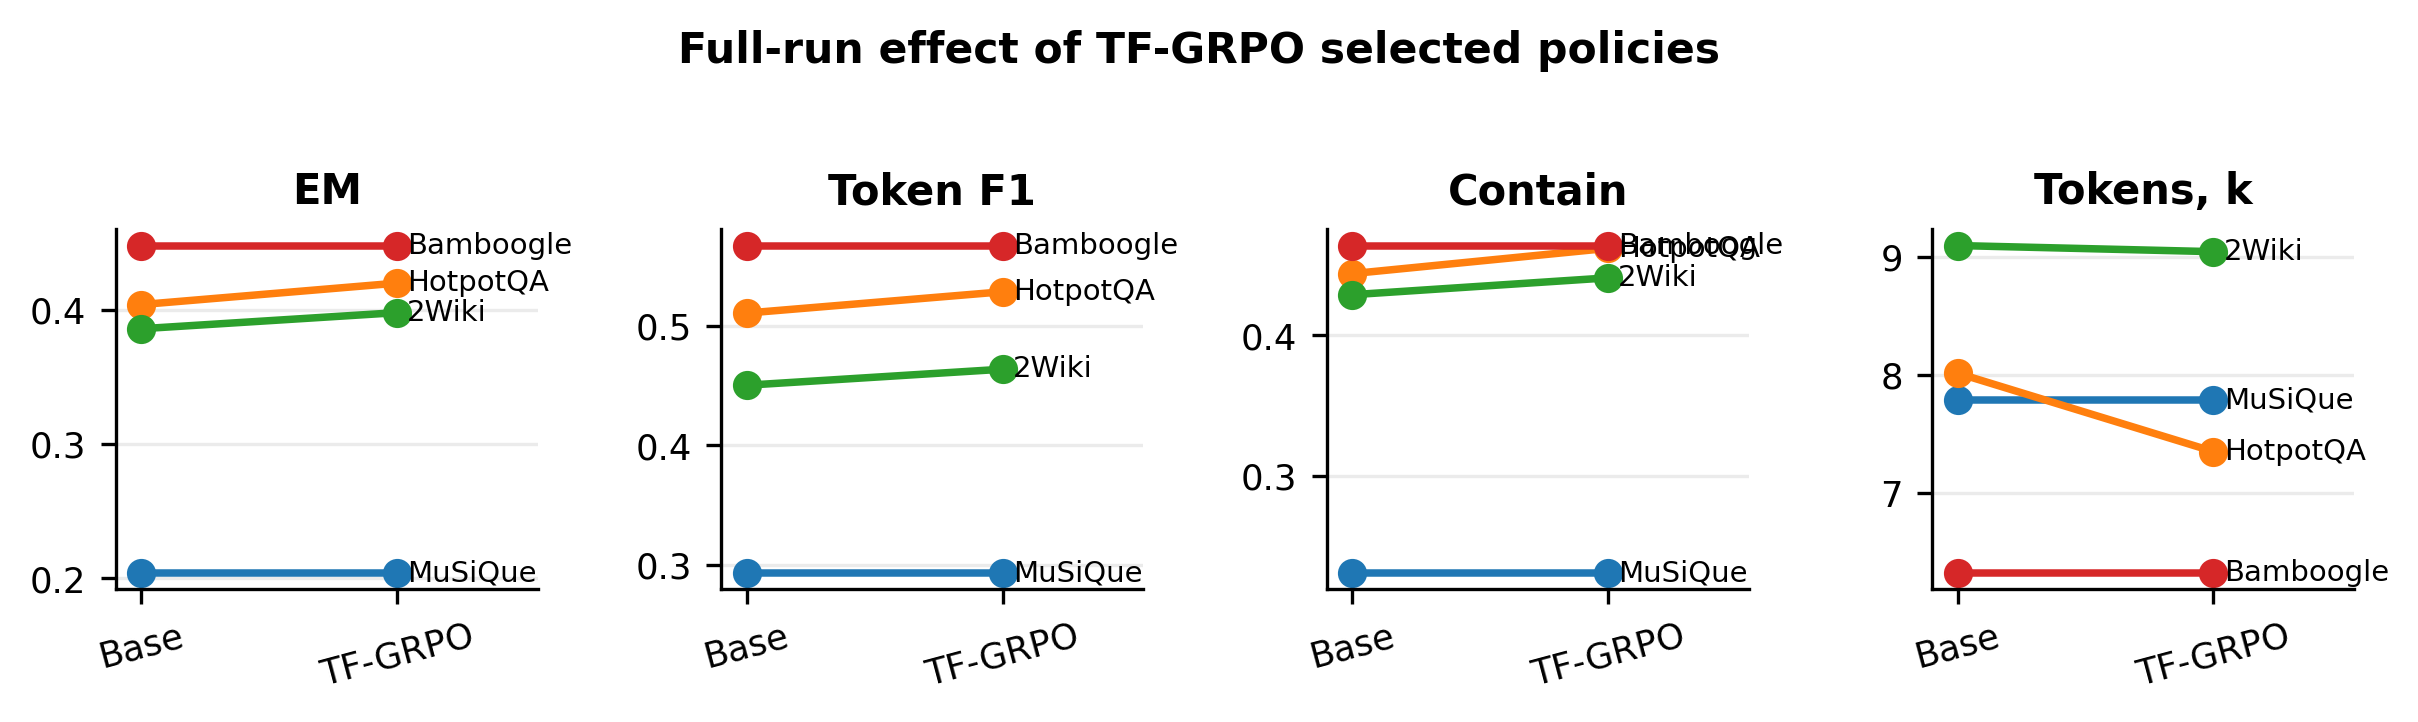
\includegraphics[width=.96\linewidth]{figs/base_tfgrpo_slope.png}
\caption{Base to TF-GRPO movement on full runs. TF-GRPO improves HotpotQA and 2Wiki, and preserves MuSiQue and Bamboogle when no better policy was validated.}
\label{fig:slope}
\end{figure}

\section{Baseline comparison}

The baseline suite uses the same top-5 no-thinking retrieval setting. AMAS3 is not the cheapest method, but it is the strongest by exact match and token-F1 across all evaluated datasets. This is the central achievement of the branch: the method substantially improves quality while staying far below the old 20k-token style of multi-agent inference.

\begin{figure}[H]
\centering
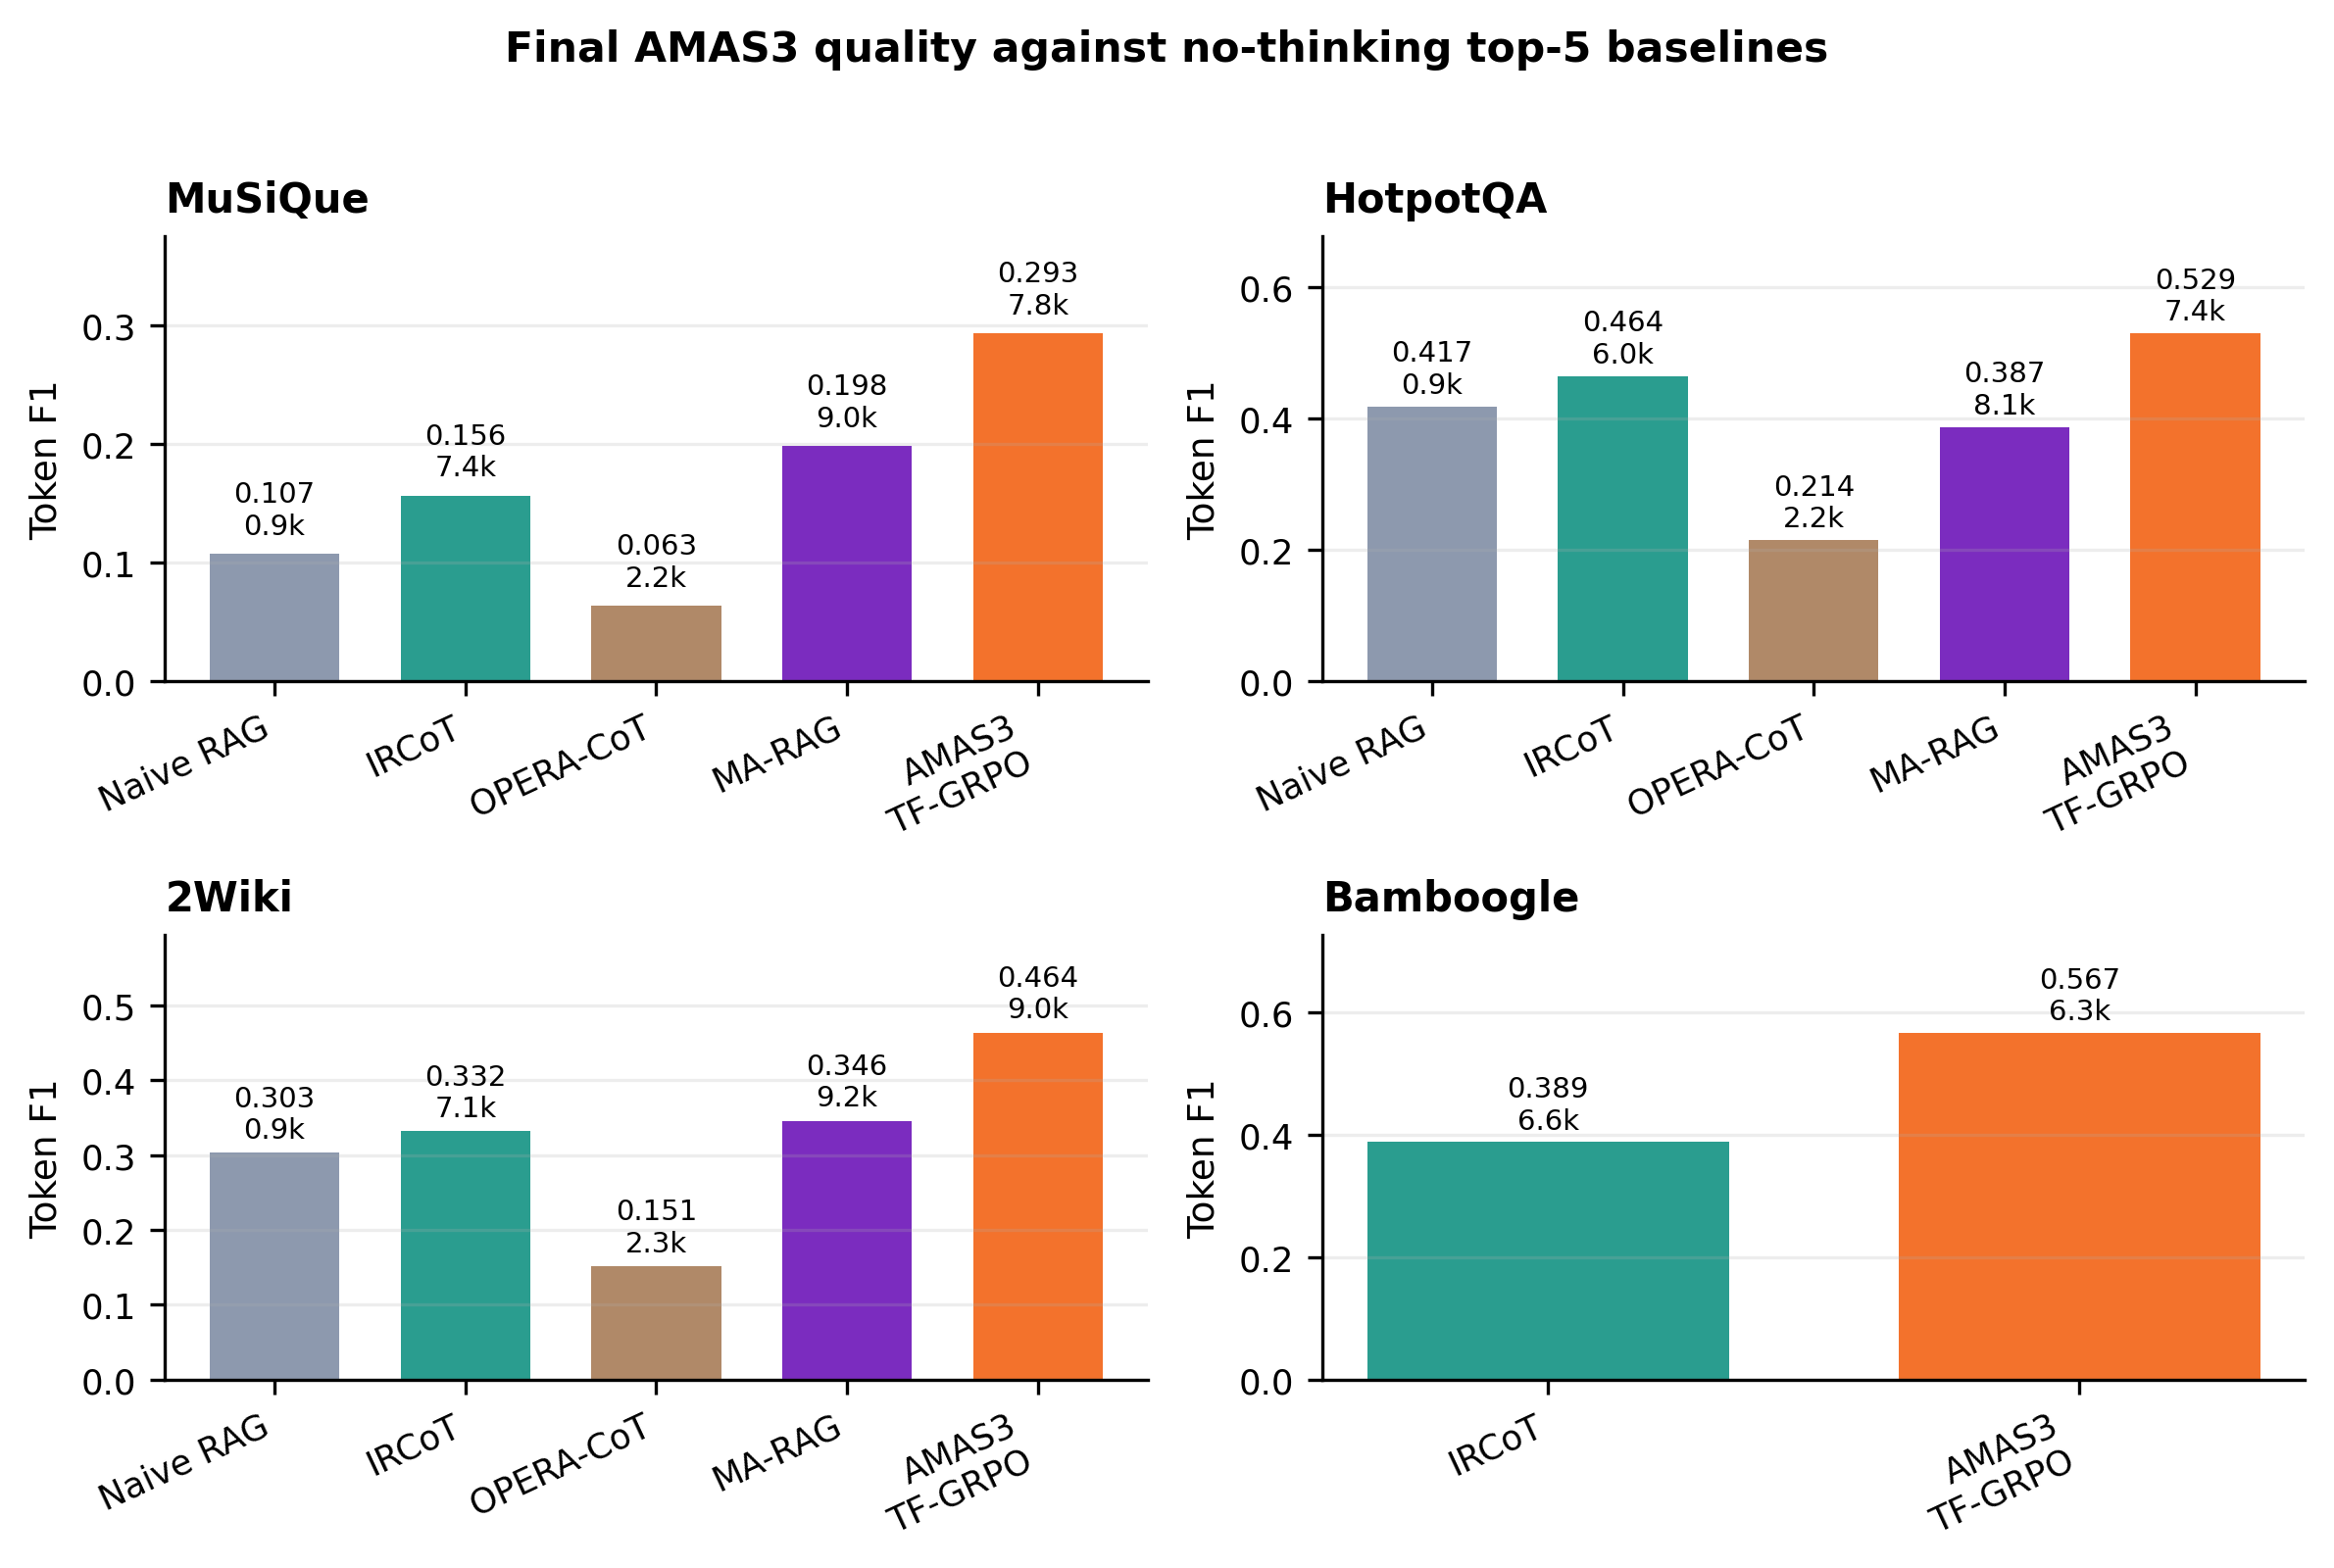
\includegraphics[width=.92\linewidth]{figs/quality_baseline_facets.png}
\caption{Token-F1 against the no-thinking top-5 baseline suite. Labels above bars show F1 and mean tokens. AMAS3 gives the strongest F1 on every dataset.}
\label{fig:baseline-facets}
\end{figure}

\begin{table}[H]
\centering
\small
\begin{tabular}{llrrrr}
\toprule
Dataset & Method & EM & F1 & Contain & Tokens \\
\midrule
\multirow{5}{*}{MuSiQue} & Naive RAG & .038 & .1073 & .079 & 881 \\
 & IRCoT & .081 & .1564 & .127 & 7409 \\
 & OPERA-CoT & .015 & .0634 & .058 & 2206 \\
 & MA-RAG & .106 & .1982 & .177 & 9029 \\
 & AMAS3 final & .204 & .2933 & .231 & 7786 \\
\midrule
\multirow{5}{*}{HotpotQA} & Naive RAG & .301 & .4174 & .377 & 887 \\
 & IRCoT & .347 & .4638 & .448 & 6046 \\
 & OPERA-CoT & .098 & .2142 & .327 & 2227 \\
 & MA-RAG & .270 & .3865 & .420 & 8067 \\
 & AMAS3 final & .420 & .5286 & .462 & 7351 \\
\midrule
\multirow{5}{*}{2Wiki} & Naive RAG & .253 & .3031 & .295 & 925 \\
 & IRCoT & .243 & .3317 & .474 & 7106 \\
 & OPERA-CoT & .046 & .1515 & .304 & 2258 \\
 & MA-RAG & .265 & .3458 & .412 & 9195 \\
 & AMAS3 final & .398 & .4638 & .441 & 9045 \\
\midrule
\multirow{2}{*}{Bamboogle} & IRCoT & .296 & .3885 & .352 & 6558 \\
 & AMAS3 final & .448 & .5673 & .464 & 6322 \\
\bottomrule
\end{tabular}
\caption{Baseline comparison. AMAS3 has the strongest EM and F1 on all four datasets. IRCoT has higher contain on 2Wiki, which indicates that it often includes the gold string in a longer answer while AMAS3 is more exact-span oriented.}
\label{tab:baselines}
\end{table}

\section{Token analysis}

The main token finding is that planner cost is not the bottleneck. The final policies spend less than 900 planner tokens per question on all datasets. The solver is the dominant consumer, followed by synthesis. This explains why the effective TF-GRPO policies either reduced synthesis context or improved solver repair, rather than trying to compress the planner further.

\begin{figure}[H]
\centering
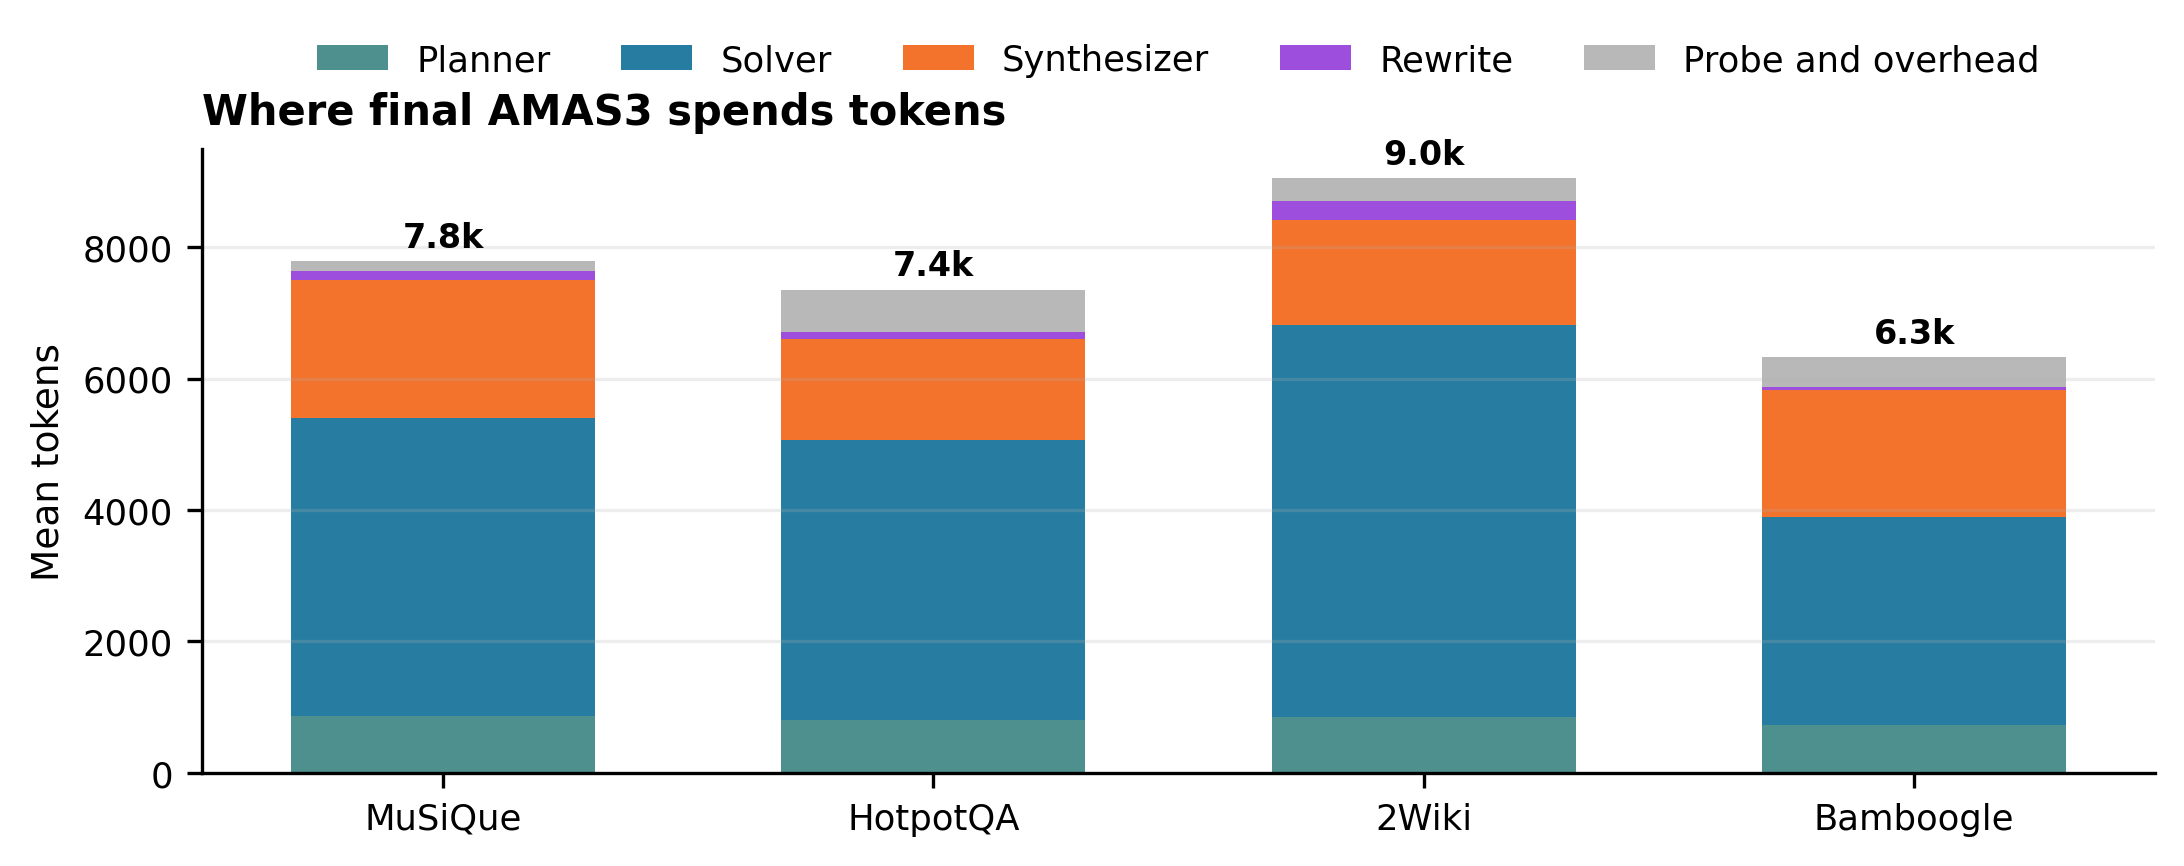
\includegraphics[width=.88\linewidth]{figs/token_components_polished.png}
\caption{Final token components. Solver calls dominate total cost, synthesis is second, and planner cost is comparatively small.}
\label{fig:tokens}
\end{figure}

\begin{table}[H]
\centering
\small
\begin{tabular}{lrrrrr}
\toprule
Dataset & Planner & Solver & Synthesizer & Rewrite & Total \\
\midrule
MuSiQue & 867 & 4528 & 2109 & 135 & 7786 \\
HotpotQA & 806 & 4265 & 1528 & 108 & 7351 \\
2Wiki & 844 & 5974 & 1592 & 298 & 9045 \\
Bamboogle & 731 & 3166 & 1923 & 56 & 6322 \\
\bottomrule
\end{tabular}
\caption{Mean actual tokens by component for the final policies. Differences between component sums and totals are probe calls and orchestration overhead.}
\label{tab:token-components}
\end{table}

\section{Dataset-level interpretation}

\paragraph{MuSiQue.}
MuSiQue is the clearest remaining weakness. AMAS3 beats all listed baselines by F1 and EM, but TF-GRPO did not improve over the new base. The train surface shows why: deeper planning and extra retrieval are better than compact synthesis for MuSiQue, but they do not solve the underlying bridge-recovery problem. Many failures are cases where an intermediate bridge answer is plausible but the final relation is mis-targeted. More synthesis tokens do not reliably fix this because the required evidence was often not recovered or not linked in the right order.

\paragraph{HotpotQA.}
HotpotQA is the cleanest success. Compact five-evidence synthesis and comparison alignment improved every metric and reduced tokens. The system moved from 0.404 EM, 0.5108 F1, and 8015 tokens to 0.420 EM, 0.5286 F1, and 7351 tokens. This is exactly the intended TF-GRPO behavior: recover quality and efficiency together by removing unnecessary synthesis context.

\paragraph{2Wiki.}
2Wiki benefited from repair and comparison alignment. The best quality variant reached 0.4711 F1 and 0.450 contain at 9506 tokens, but the selected policy achieved 0.4638 F1 and 0.441 contain at 9045 tokens. The selected policy is therefore the better research point for the stated objective because it improves over base while staying closer to the efficiency target.

\paragraph{Bamboogle.}
Bamboogle retained the compact base. The final score is 0.448 EM, 0.5673 F1, and 0.464 contain at 6322 tokens, above the available full baseline. The dataset has only 125 questions, so the search evidence did not justify a more complex policy. Preserving the base is a valid outcome of the policy search.

\section{Limitations and next steps}

The current method is a strong training-free policy optimizer, but it is not yet a complete solution to MuSiQue-style bridge reasoning. The residual failure modes are concentrated in three places. First, bridge-conditioned retrieval is still brittle when the first hop produces a plausible but wrong entity. Second, solver fan-out remains expensive on 2Wiki because comparison questions often require multiple candidate-specific retrievals. Third, contain and exact-span behavior diverge on some datasets: AMAS3 is better at exact answers, while IRCoT sometimes has higher contain by producing longer strings.

The next technical step should not be more generic policy search. It should be targeted system work: improve bridge query construction for MuSiQue, reduce solver fan-out with earlier candidate pruning for 2Wiki, and add stricter final-target checks that reject bridge answers before synthesis.

\section{Conclusion}

AMAS3 now has a reproducible training-free optimization pipeline: experience-library collection, mixed train rollouts, group-relative reward scoring, policy selection, and full held-out evaluation. The final system improves over all available no-thinking top-5 baselines in EM and token-F1, while staying in the 6.3k to 9.0k token range. TF-GRPO gives real full-run gains on HotpotQA and 2Wiki, and it correctly avoids changing MuSiQue and Bamboogle when the searched alternatives do not validate. The branch therefore establishes a credible adaptive RAG baseline for the thesis: better than the static baselines, efficient enough for large runs, and transparent enough to analyze scientifically.

\end{document}
